\documentclass[12pt, a4paper]{ctexart}

\usepackage{fancyhdr}
\pagestyle{fancy}
\fancyhead{}
\renewcommand{\headrulewidth}{1pt}
\renewcommand{\headwidth}{\textwidth}
\fancyhead[L]{\leftmark}
\fancyhead[R]{\thepage}
\fancyfoot{}

\fancypagestyle{plain}{
\fancyhead{}
\renewcommand{\headrulewidth}{1pt}
\fancyfoot{}
\fancyhead[L]{北京大学基础物理实验报告}
\fancyhead[R]{唐晨宇}
}
\usepackage[colorlinks,linkcolor=red,urlcolor = blue]{hyperref}
\usepackage{booktabs}
\usepackage{graphicx}
\usepackage{amsmath}
\usepackage{mathcomp}
\usepackage{mathabx}
\usepackage{enumitem}
\usepackage[top=1.2in, bottom=1.2in, left=0.95in, right=0.95in]{geometry}
\usepackage{circuitikz}
\usepackage{multirow}
\usepackage{wrapfig}
\usepackage{textcomp}
\usepackage{diagbox}

\ctexset{
    section={   
        name={,},
        number={\chinese{section}},
        format=\heiti\raggedright
    },
    subsection={   
        name={(,)},
        number={\chinese{subsection}},
        format=\heiti
    }
}

\begin{document}
\title{直流电桥测量电阻\&非平衡电桥测量铂电阻的温度系数}
\author{唐晨宇 \quad 2300934207}
\date{2024年4月}

\maketitle
\footnotetext{本实验报告计算过程中涉及的不确定度均多保留一位有效数字,以下同理.}

\tableofcontents

\clearpage

\section*{实验仪器}

\begin{itemize}
    \item 待测电阻$R_{x1}$
    \item $10k\Omega$色环电阻两个
    \item $1k\Omega$和$100\Omega$精密电阻各两个,允差$0.1\%$
    \item VC9806+型数字式万用表两块,200mV及20V挡允差$\pm (0.05\% + 3 \text{个字})$,$20k\Omega$挡允差$\pm (0.02\% + 5\text{个字})$
    \item UTP3313TFL-II稳压电源
    \item 三线式铂电阻传感器
    \item NTY-2A型数字式温度计
    \item AC5/2型直流指针式检流计,灵敏度$S_i= 1.3 \times 10^{-6} A$/格
    \item ZX96型直流电阻器,其接触电阻为$R_0 = (12 \pm 5)m\Omega$,各量程允差见表\ref{t2}
    \item 电位器,零值电阻为$R_{0(0)} = 3.05\Omega$
    \item $50\sim 500g$砝码,精度$0.005\%$
    \item 实验室提供的电热杯和保温杯
\end{itemize}

经万用表测量得各电阻实际阻值如表\ref{t1}所示.
规定若标称值误差在1\textperthousand 以内,则计算时取标称值.
另外测量得$R_{x1} = 32.80\Omega$.

\begin{table}[hbtp]
    \centering
    \begin{tabular}{|c|c|c|}
    \hline
    \multirow{2}{*}{标称值/$\Omega$} & \multicolumn{2}{c|}{测量值/$\Omega$} \\
    \cline{2-3}
      & $R_A$ & $R_B$ \\
    \hline
    100 & 99.95 &99.96 \\
    \hline
    1k & 0.9999k & 1.0000k \\
    \hline
    10k & 9.956k &10.059k \\
    \hline
    \end{tabular}
    \caption{各电阻实测值}
    \label{t1}
\end{table}

\begin{table}[hbtp]
    \centering
    \begin{tabular}{ccccccc}
    \toprule
    挡位/$\Omega$ & $\times 10k$ & $\times 1k$ & $\times 100$ & $\times 10$ & $\times 1$ & $\times 0.1$ \\
    \midrule
    允差$e$   & $\pm 0.10\%$ & $\pm 0.10\%$ & $\pm 0.10\%$ & $\pm 0.10\%$ & $\pm 0.50\%$ & $\pm 2\%$ \\
    \bottomrule
    \end{tabular}
    \caption{ZX96型直流电阻器允差}
    \label{t2}
\end{table}

\clearpage

\section{平衡电桥}

\begin{wrapfigure}{l}{2.5in}
    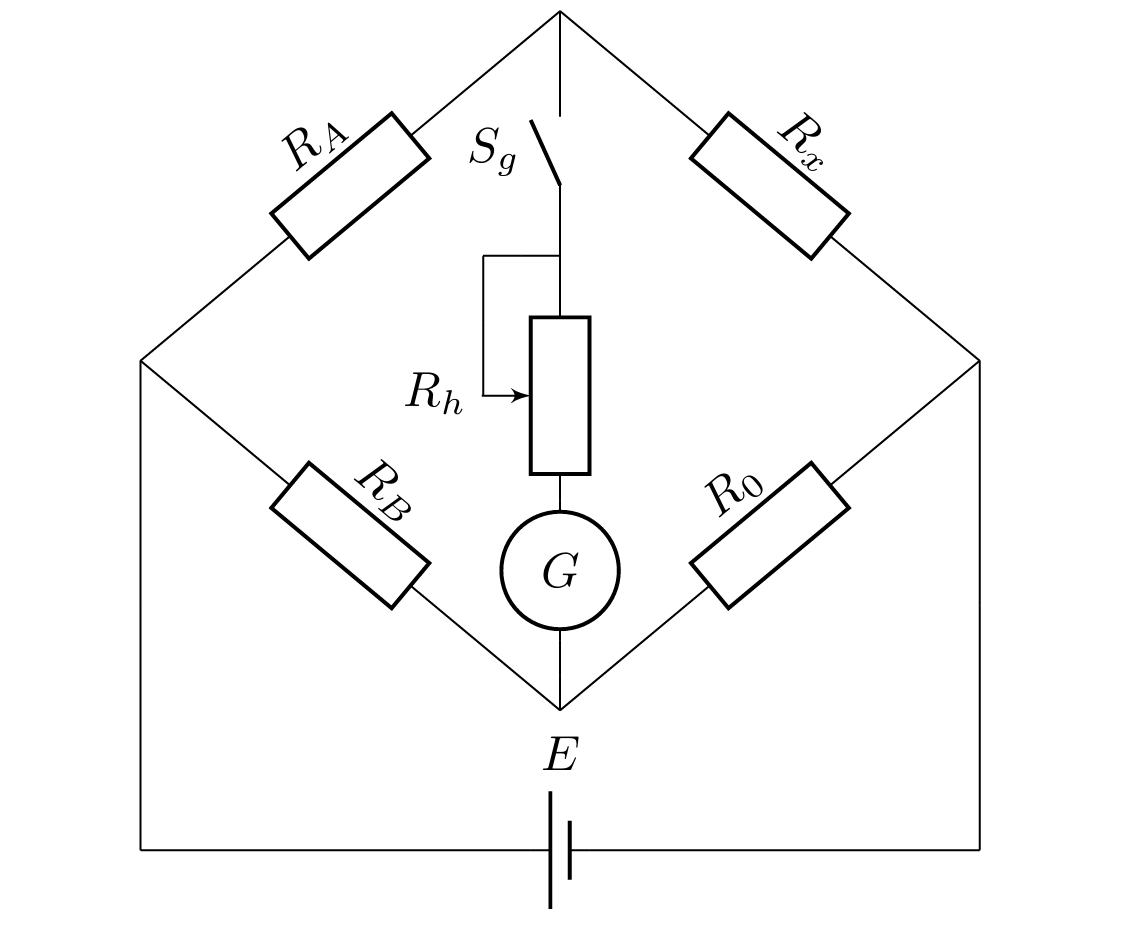
\includegraphics[width=2.5in]{figure/circuit_balenced.png}
    \caption{平衡电桥}
    \label{fig1}
\end{wrapfigure}

电路如左图\ref{fig1}所示,各数据见表\ref{t2},表中$10k/10k$组为利用交换桥臂法测得的数据($10k\Omega$电阻为色环电阻,真实值与标称值误差较大),
其中下标为1的一行电路连接与图\ref{fig1}相符,有
$R_x = \sqrt{R_{01} R_{02}}$.

对于前两组数据,有
\begin{equation*}
    R_x = \frac{R_A}{R_B} R_0
\end{equation*}
各组数据中有
\begin{equation*}
    S = \frac{\Delta n }{\frac{\Delta R_0}{R_0}}
\end{equation*}

\begin{table}[hbtp]
    \centering
    \caption{平衡电桥测量数据}
    \begin{tabular}{c|c|c|c|ccccc|c}
        \toprule
        i & $E/V$ & $R_h/\Omega$ & $R_A/R_B (\Omega/\Omega)$ & $R_0/\Omega$ & $R_0'/\Omega$ & $\Delta R_0/\Omega$ & $\Delta n$ & $S$ & $R_x$ \\
        \hline
        1 & \multirow{5}{*}{1.9919} &\multirow{4}{*}{3.05} & 100/100 & 32.8 & 32.9 & 0.1 & 8.7 & 2853.6 & 32.8 \\
        \cline{1-1}
        \cline{4-10}
        2 &  &  & 100/1k & 328.3 & 329.3 & 1.0 & 2.3 & 755.09 & 32.83 \\
        \cline{1-1}
        \cline{4-10}
        \multirow{2}{*}{3} &  &  & \multirow{2}{*}{10k/10k} & $R_{01} = 33.2$ & 33.5 & 0.3 & 3.7 & 40.95 & \multirow{2}{*}{33.05} \\
        \cline{5-9}
          &  &  &  & $R_{02} = 32.9$ & 33.2 & 0.3 & 2.1 & 23.03 &  \\
        \cline{1-1}
        \cline{3-10}
        4 &  & 3012 & 100/100 & 33.0 & 31.0 & 2.0 & 2.9 & 47.85 & 33.0 \\
        \bottomrule
    \end{tabular}
    \label{t3}
\end{table}

$R_0$允差根据表\ref{t2}计算,$R_A$和$R_B$允差为$0.1\%$,假设误差均匀分布.
由待测电阻计算公式可得
\begin{equation*}
    \sigma_{R_x}' = R_x \sqrt{(\frac{e_{R_A}}{\sqrt{3}R_A})^2 + (\frac{e_{R_B}}{\sqrt{3}R_B})^2 + (\frac{e_{R_0}}{\sqrt{3}R_0})^2}
\end{equation*}
检流计分辨率为0.2格,故由电桥灵敏度限制带来的误差为
\begin{equation*}
    \delta R_x = \frac{0.2R_x}{S}
\end{equation*}
故最终不确定度为
\begin{equation*}
    \sigma_{R_x} = \sqrt{(\sigma_{R_x}')^2 + (\delta R_x)^2}
\end{equation*}
相对不确定度
\begin{equation*}
    \frac{\sigma_{R_x}}{R_x} = \sqrt{(\frac{e_{R_A}}{\sqrt{3}R_A})^2 + (\frac{e_{R_B}}{\sqrt{3}R_B})^2 + (\frac{e_{R_0}}{\sqrt{3}R_0})^2 + (\frac{0.2}{S})^2}
\end{equation*}
在交换桥臂法中
\begin{gather*}
    \delta R_{0i} = \frac{0.2R_{0i}}{S}\\
    \sigma_{R_{0i}} = \sqrt{(\frac{e_{R_0}}{\sqrt{3}})^2 + (\delta R_{0i})^2}
\end{gather*}
其中$i = 1,2$.故最终结果不确定度为
\begin{equation*}
    \sigma_{R_x} = \sqrt{(\frac{\partial R_x}{\partial R_{01}})^2 \sigma_{R_{01}}^2 + (\frac{\partial R_x}{\partial R_{02}})^2 \sigma_{R_{02}}^2} = \frac{R_x}{2}\sqrt{(\frac{\sigma_{R_{01}}}{R_{01}})^2 + (\frac{\sigma_{R_{02}}}{R_{02}})^2}
\end{equation*}
利用以上结论计算得到最终结果见表\ref{t4}.
\begin{table}[htbp]
    \centering
    \begin{tabular}{cccccccccc}
        \toprule
        i & $R_A/R_B(\Omega/\Omega)$ & $e_{R_A}/\Omega$ & $e_{R_B}/\Omega$ & $R_0/\Omega$ & $e_{R_0}/\Omega$ & $\sigma_{R_x}'$ & $\delta R_x$ & $\sigma_{R_x}$ & 测量结果 \\
        \midrule
        1 & 100/100 & 0.1 & 0.1 & 32.8 & 0.056 & 0.042 & 0.0023 & 0.05 & $32.80 \pm 0.05$ \\
        \hline
        2 & 100/1k & 0.1 & 1 & 328.3 & 0.366 & 0.035 & 0.009 & 0.04 & $32.83 \pm 0.04$ \\
        \hline
        \multirow{2}{*}{3} & \multirow{2}{*}{10k/10k} & — & — & 33.2 & 0.049 & — & 0.17 & 0.18 & \multirow{2}{*}{$33.05 \pm 0.18$} \\
        \cline{3-9}
          &  & — & — & 32.9 & 0.058 & — & 0.29 & 0.30 &  \\
        \hline
        4 & 100/100 & 0.1 & 0.1 & 33.0 & 0.045 & 0.037 & 0.14 & 0.15 & $33.00 \pm 0.15$ \\
        \bottomrule
    \end{tabular}
    \caption{各组数据及结果不确定度}
    \label{t4}
\end{table}

从表中数据可以看出,1组和2组数据各电阻允差产生的不确定度占主要地位,而第3组和第4组数据中则为电桥灵敏度限制产生的不确定度主要影响结果误差.
其中3组电桥灵敏度较低的原因主要是两定值桥臂电阻不等且阻值远大于待测电阻,而4组电桥灵敏度较低的原因主要是与检流计串联的保护电阻$R_h$较大.

由电桥的基尔霍夫方程可以推得电桥灵敏度的理论计算公式为
\begin{equation*}
    S = \frac{S_i \cdot E}{R_A + R_B + R_x + R_0 + R_h(2 + \frac{R_A}{R_x} + \frac{R_0}{R_B})}
\end{equation*}
由于实验精度有限,对各组电桥灵敏度理论值分别进行计算没有太大意义,但可以看到灵敏度与$R_A,R_B,R_h$呈负相关,与实验数据相符.

整体结果在三位有效数字的精度下保持一致,但3组和4组测量结果与数字表测量结果相比存在0.2\textperthousand 的偏差,可能是由于电桥灵敏度限制对结果误差的影响仍在我们测量计算得到的不确定度之上.

\begin{wrapfigure}{r}{2.5in}
    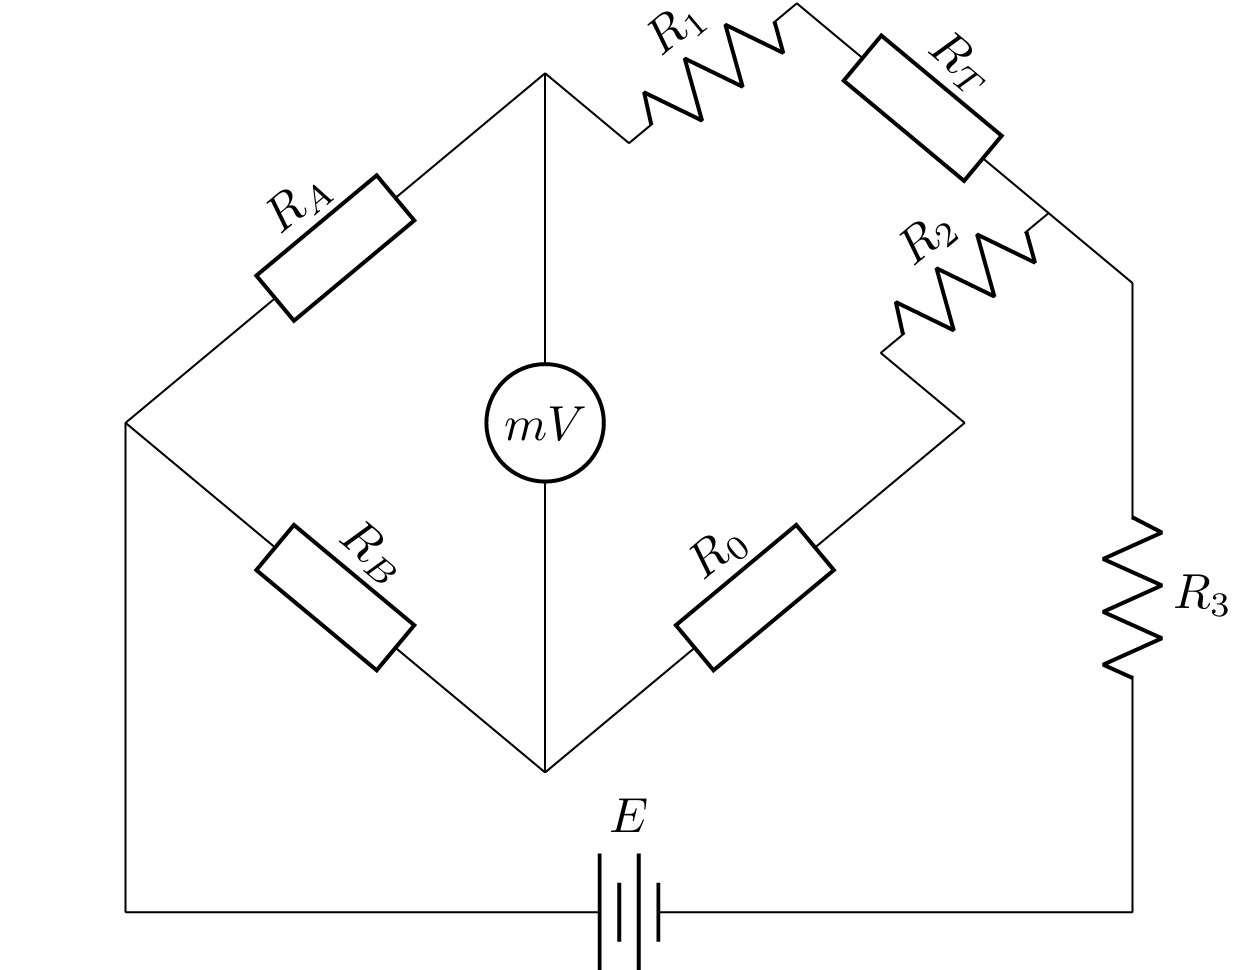
\includegraphics[width=2.5in]{figure/circuit_unbalenced.png}
    \caption{非平衡电桥}
    \label{fig2}
\end{wrapfigure}

\section{非平衡电桥}

电路连接如左图\ref{fig2}所示\footnotemark,其中美式折线型电阻$R_3$,$R_4$和$R_5$代表由于电路连接导致的接触电阻及导线电阻,应用三线接法可有效减小其对电路产生的影响.
\footnotetext{此处恒压源与主电路之间以一双刀单掷开关连接,可等效忽略.}
$R_T$为热敏铂电阻传感器,与温度计共同浸没于温度可调的水中.
左侧两定值电阻为10k/10k(非精确值),下方$R_0$取冰点时电桥平衡电阻,$R_0 = 99.8\Omega$,电源电压取$E = 19.024V$.

\clearpage

测得水温$T$与桥路中毫伏表示数值$U_{out}$关系如表\ref{t5},线性拟合如图\ref{fig3}.

\begin{table}[htbp]
    \centering
    \begin{tabular}{cccccccccc}
        \toprule
        $T/^{\circ} C$ & 0.54 & 21.40 & 40.75 & 50.18 & 60.40 & 70.40 & 80.00 & 90.45 & 99.95 \\
        \midrule
        $U_{out}/mV$ & 0.04 & 13.87 & 27.68 & 34.42 & 41.67 & 48.69 & 55.37 & 62.73 & 69.29 \\
        \bottomrule
    \end{tabular}
    \caption{非平衡电桥测量铂电阻传感器$T-U_{out}$数据表}
    \label{t5}
\end{table}

\begin{figure}[htbp]
    \centering
    \caption{$T-U_{out}$拟合曲线}
    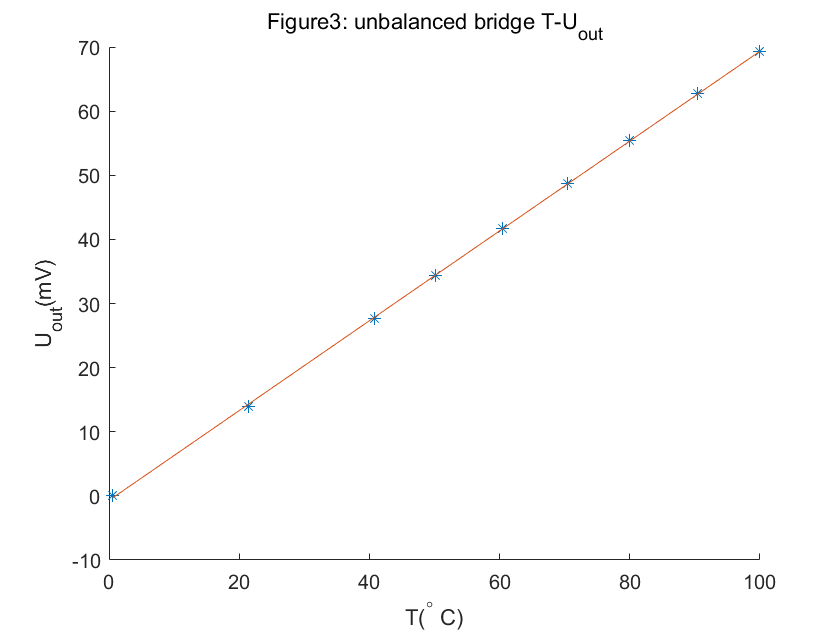
\includegraphics[width=4in]{figure/T-U_out figure.png}
    \label{fig3}
\end{figure}

拟合结果为
\begin{align*}
    U_{out}(mV) &= 0.7006T(^{\circ} C) - 0.7093 \\
    r &= 0.99995
\end{align*}
即拟合斜率为$k = 0.7006 mV/^{\circ}C$,线性度为0.6\%,其中最大偏差出现于第二组数据.
由拟合带来的不确定度为
\begin{equation*}
    \sigma_{kA} = k \sqrt{\frac{1/r^2 - 1}{n - 2}} = 0.0027 mV/^{\circ}C
\end{equation*}
又有电压表允差贡献的不确定度,电压表允差最大值为
\begin{equation*}
    e = (69.29 \times 0.05\% + 0.03)mV = 0.07mV
\end{equation*}
故传递至斜率
\begin{equation*}
    \sigma_{kB} = \frac{e/\sqrt{3}}{\sqrt{\sum_{i}(T_i - \bar{T})^2}} = 0.0005 mV/^{\circ}C
\end{equation*}
最终合成误差
\begin{equation*}
    \sigma_k = \sqrt{\sigma_{kA}^2 + \sigma_{kB}^2} = 0.0028 mV/^{\circ}C
\end{equation*}

理论计算表明
\begin{equation*}
    U_{out} = E (\frac{R_T}{R_T + R_A} - \frac{R_0}{R_0 + R_B})
\end{equation*}
当电路参数满足$R_A \gg R_T$时,$U_{out}$与$R_T$大致呈线性关系,即$R_A + R_T \approx R_A$.
又有
\begin{equation*}
    R_T = R_{T0}(1 + A_1 T)
\end{equation*}
开始铂电阻温度为冰点时电桥满足
\begin{equation*}
    \frac{R_A}{R_B} = \frac{R_{T0}}{R_0}
\end{equation*}
结合以上三式得
\begin{equation*}
    \Delta U_{out} = \frac{E}{R_B}R_0 A_1 \Delta T
\end{equation*}
即
\begin{equation*}
    A_1 = \frac{k R_B}{E R_0} = 3.712 \times 10^{-3} {^{\circ} C}^{-1}
\end{equation*}
其中$R_B$取表\ref{t1}中测量值,其允差
\begin{equation*}
    e_{R_B} = (10.059 \times 0.02\% + 0.005)k\Omega = 0.008 k\Omega
\end{equation*}
输出电压允差
\begin{equation*}
    e_E = (19.024 \times 0.05\% + 0.003)V = 0.013 V
\end{equation*}
电阻箱$R_0$允差
\begin{equation*}
    e_{R_0} = (90 \times 0.1\% + 9 \times 0.5\% + 0.8 \times 2\%)\Omega = 0.151\Omega
\end{equation*}
故铂电阻温度系数不确定度为
\begin{equation*}
    \sigma_{A_1} = A_1 \sqrt{(\frac{\sigma_k}{k})^2 + (\frac{e_{R_B}}{\sqrt{3} R_B})^2 + (\frac{e_{R_0}}{\sqrt{3} R_0})^2 + (\frac{e_{E}}{\sqrt{3} E})^2} = 0.016 \times 10^{-3} {^{\circ}C}^{-1}
\end{equation*}
因此该铂电阻温度系数测量值为
\begin{equation*}
    A_1 \pm \sigma_{A_1} = (3.712 \pm 0.016)\times 10^{-3} {^{\circ}C}^{-1}
\end{equation*}
实验室给出的理论值为
\begin{equation*}
    A_1 = 3.85 \times 10^{-3} {^{\circ}C}^{-1}
\end{equation*}
可见测量值相对标准值偏小.

电桥灵敏度定义为
\begin{equation*}
    K = \frac{\Delta U_{out}}{\Delta T} \approx k = 0.7006 mV/^{\circ}C
\end{equation*}
相应有分辨率为
\begin{equation*}
    D = \frac{1}{k} = 0.014{^{\circ}C}/0.01mV
\end{equation*}

\section{应变片实验}
\subsection{quarter bridge}

\begin{wrapfigure}{l}{2.5in}
    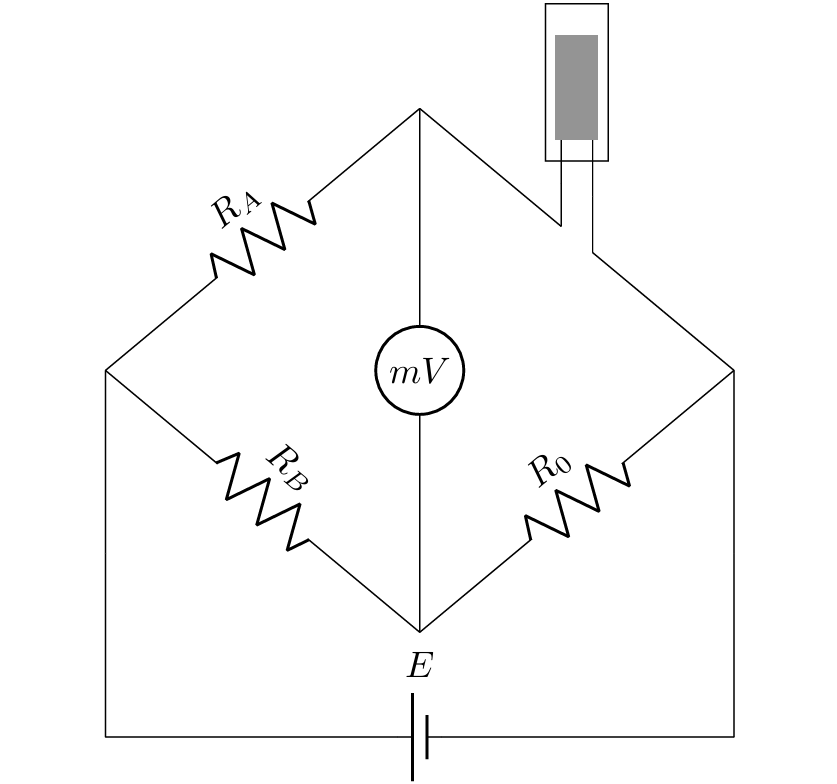
\includegraphics[width=2.5in]{figure/quarter bridge.png}
    \caption{1/4桥电路}
    \label{fig4}
\end{wrapfigure}

实验电路如左图\ref{fig4}所示,其中$R_A/R_B = 100/1k$,电源电压取$E = 10.018V$.
粘有应变片的平行梁上除去装置本身之外的负载为零时调节电桥平衡,此时$R_0 = 3733.9\Omega$.
取不同质量的砝码作为负载,测量得到应变片等效受力$F$(单位为克力)与输出电压$U_{out}$关系如表\ref{t6},线性拟合如图\ref{fig5}.

拟合结果为
\begin{align*}
    U_{out}(mV) &= 0.00205F(gf) + 0.02110 \\
    r &= 0.9994
\end{align*}
即电桥灵敏度
\begin{equation*}
    K_{1/4} = \frac{\Delta U_{out}}{\Delta F} \approx 0.002mV/gf
\end{equation*}

\begin{table}[htbp]
    \centering
    \begin{tabular}{cccccccccc}
        \toprule
        $F/gf$ & 0 & 50 & 100 & 150 & 200 & 250 & 300 & 400 & 500 \\
        \midrule
        $U/mV$ & 0.00 & 0.13 & 0.22 & 0.33 & 0.44 & 0.53 & 0.64 & 0.83 & 1.02 \\
        \bottomrule
    \end{tabular}
    \caption{1/4桥测量$F-U_{out}$关系数据}
    \label{t6}
\end{table}
\begin{figure}[htbp]
    \centering
    \caption{1/4桥$F-U_{out}$拟合曲线}
    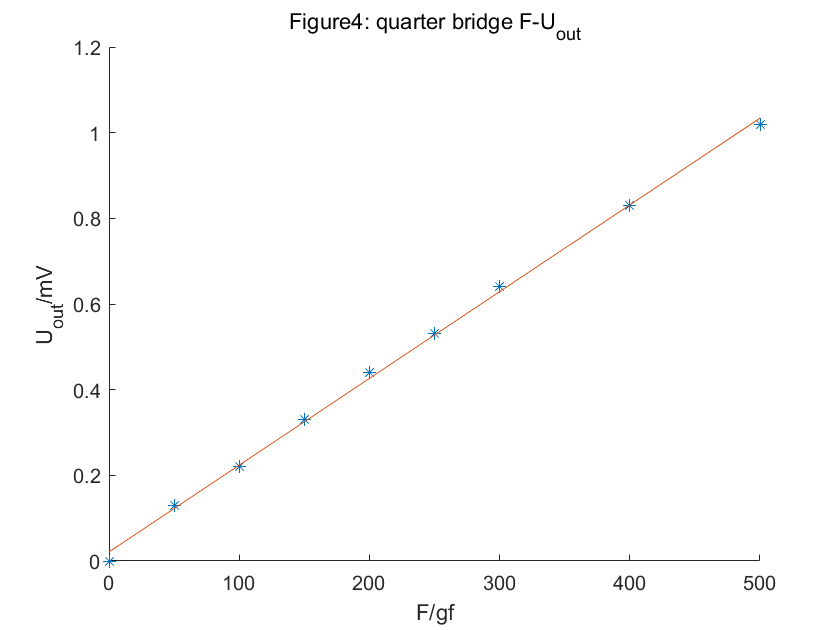
\includegraphics[width=3.9in]{figure/quarter bridge F-U_out figure.png}
    \label{fig5}
\end{figure}
电桥分辨率
\begin{equation*}
    D_{1/4} = \frac{1}{K_{1/4}} = 4.9gf/0.01mV
\end{equation*}

由拟合带来的不确定度为
\begin{equation*}
    \sigma_{kA} = k\sqrt{\frac{1/r^2 - 1}{n - 2}} = 2.7\times 10^{-5}mV/gf
\end{equation*}
电压表允差最大值为
\begin{equation*}
    e = (1.02 \times 0.05\% + 0.03) mV = 0.03051mV
\end{equation*}
故电压表允差贡献的不确定度为
\begin{equation*}
    \sigma_{kB} = \frac{e/\sqrt{3}}{\sqrt{\sum_i (F_i - \bar{F})^2}} = 3.7 \times 10^{-5}mV/gf
\end{equation*}
最终合成不确定度
\begin{equation*}
    \sigma_k = \sqrt{\sigma_{kA}^2 + \sigma_{kB}^2} = 5 \times 10^{-5} mV/gf
\end{equation*}

利用该电路测量一台iPhone15的质量,输出电压$U_1 = 0.37mV$,代入拟合公式得$m_1 = 170g$.
不确定度
\begin{equation*}
    \sigma_{m_1} = m_1 \sqrt{(\frac{e_{U_1}}{\sqrt{3}U_1})^2 + (\frac{\sigma_k}{k})^2} = 9g
\end{equation*}
即称量结果为$m_1 \pm \sigma_{m_1} = (170 \pm 9)g$

\subsection{half bridge}

\begin{wrapfigure}{l}{2.5in}
    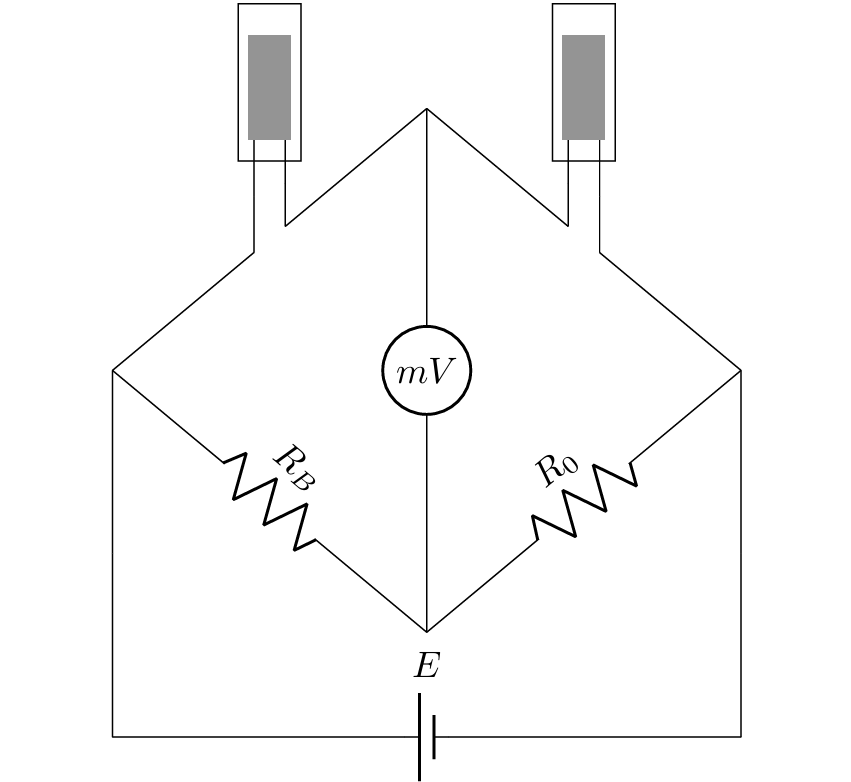
\includegraphics[width=2.5in]{figure/half bridge.png}
    \caption{半桥电路}
    \label{fig6}
\end{wrapfigure}

实验电路如左图\ref{fig6}所示,其中上方桥路为两同接线颜色应变片(阻值分别与平行梁负载成正相关、负相关),二者串联,中间引出第三条导线,导线上连有一小电阻.
电源电压同上,$R_B$取$1k\Omega$精密电阻,零负载时尽量调平电桥,此时$R_0 = 1006.6\Omega$.
各项数据处理同1/4桥,测量结果如表\ref{t7},线性拟合如图\ref{fig7}.

拟合结果为
\begin{align*}
    U_{out}(mV) &= 0.00581F(gf)- 0.01969 \\
    r &= 0.9994
\end{align*}
即电桥灵敏度
\begin{equation*}
    K_{1/2} = \frac{\Delta U_{out}}{\Delta F} = 0.006mV/gf
\end{equation*}
电桥分辨率
\begin{equation*}
    D_{1/2} = \frac{1}{K_{1/2}} = 1.7gf/0.01mV
\end{equation*}

\begin{table}[htbp]
    \centering
    \begin{tabular}{cccccccccc}
        \toprule
        $F/gf$ & 0 & 50 & 100 & 150 & 200 & 250 & 300 & 400 & 500 \\
        \midrule
        $U/mV$ & 0.05 & 0.23 & 0.54 & 0.83 & 1.13 & 1.44 & 1.73 & 2.32 & 2.89 \\
        \bottomrule
    \end{tabular}
    \caption{半桥测量$F-U_{out}$关系数据}
    \label{t7}
\end{table}

\begin{figure}[htbp]
    \centering
    \caption{半桥$F-U_{out}$拟合曲线}
    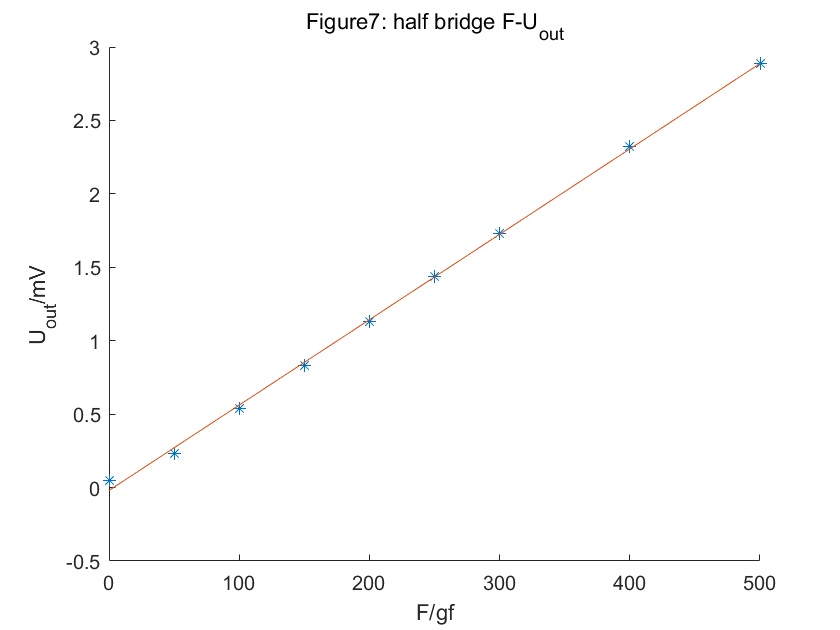
\includegraphics[width=4in]{figure/half bridge F-U_out.png}
    \label{fig7}
\end{figure}

算得斜率不确定度
\begin{equation*}
    \sigma_k = \sqrt{(k\sqrt{\frac{1/r^2-1}{n-2}})^2 + (\frac{e/\sqrt{3}}{\sqrt{\sum_i (F_i - \bar{F})^2}})^2} = 9 \times 10^{-5}mV/gf
\end{equation*}

利用该电路测量一台iPhone15的质量,输出电压$U_2 = 0.98mV$,代入拟合公式得$m_2 = 172g$.
不确定度
\begin{equation*}
    \sigma_{m_2} = m_2 \sqrt{(\frac{e_{U_2}}{\sqrt{3}U_2})^2 + (\frac{\sigma_k}{k})^2} = 4g
\end{equation*}
即称量结果为$m_1 \pm \sigma_{m_1} = (172 \pm 4)g$

\subsection{full bridge}

实验电路如图\ref{fig8}所示,其中上方桥路为两同接线颜色应变片(阻值分别与平行梁负载成正相关、负相关),二者串联,中间引出第三条导线,导线上连有一小电阻.
下方桥路同理,其中阻值与负载正相关的两片应变片处于电桥对角位置,电源电压同上.
各项数据处理同1/4桥,测量结果如表\ref{t8},线性拟合如图\ref{fig9}.

拟合结果为
\begin{align*}
    U_{out}(mV) &= 0.01188F(gf) + 28.74748 \\
    r &= 0.999995
\end{align*}
即电桥灵敏度
\begin{equation*}
    K_{1} = \frac{\Delta U_{out}}{\Delta F} = 0.012mV/gf
\end{equation*}
电桥分辨率
\begin{equation*}
    D_{1/2} = \frac{1}{K_{1}} = 0.84gf/0.01mV
\end{equation*}

\begin{table}[htbp]
    \centering
    \begin{tabular}{cccccccccc}
        \toprule
        $F/gf$ & 0 & 50 & 100 & 150 & 200 & 250 & 300 & 400 & 500 \\
        \midrule
        $U/mV$ & 28.75 & 29.35 & 29.93 & 30.53 & 31.11 & 31.72 & 32.31 & 33.50 & 34.69 \\
        \bottomrule
    \end{tabular}
    \caption{半桥测量$F-U_{out}$关系数据}
    \label{t8}
\end{table}

\begin{figure}[htbp]
    \centering
    \caption{半桥$F-U_{out}$拟合曲线}
    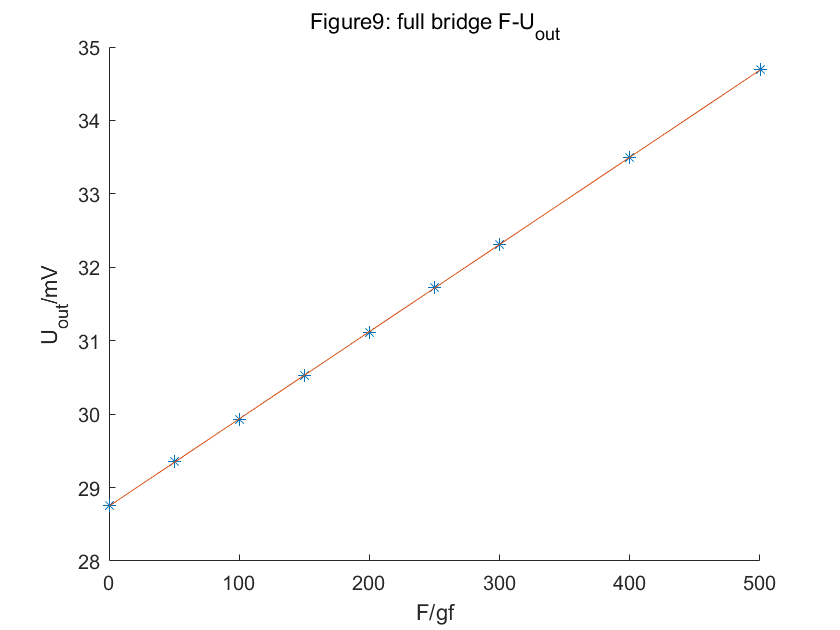
\includegraphics[width=4in]{figure/full bridge F-U_out.png}
    \label{fig9}
\end{figure}

\begin{wrapfigure}{l}{2.5in}
    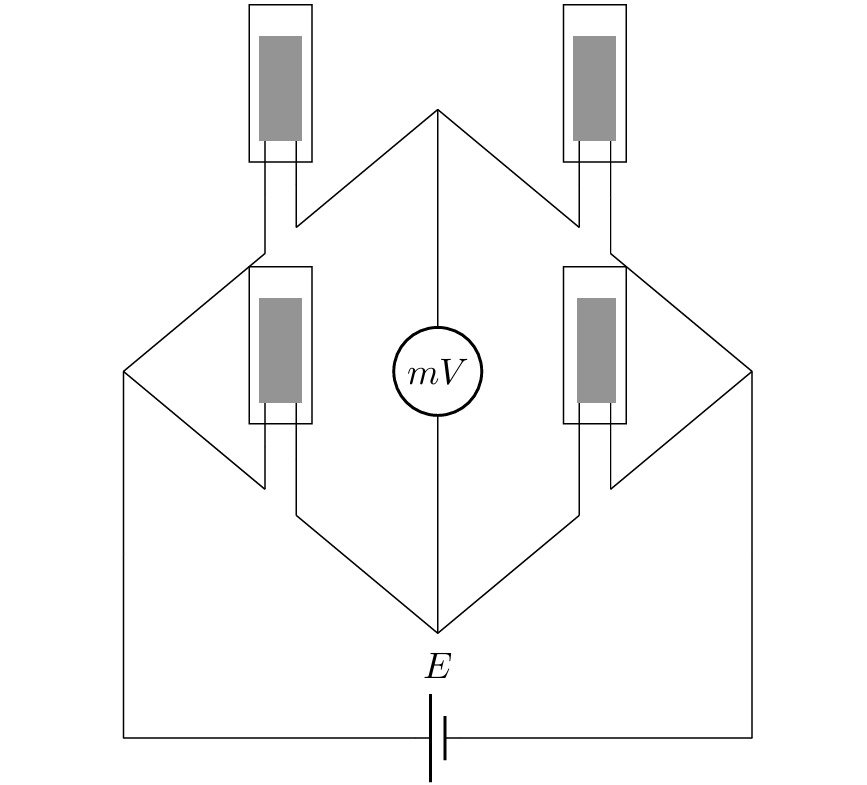
\includegraphics[width=2.5in]{figure/full bridge.png}
    \caption{半桥电路}
    \label{fig8}
\end{wrapfigure}

算得斜率不确定度
\begin{equation*}
    \sigma_k = \sqrt{(k\sqrt{\frac{1/r^2-1}{n-2}})^2 + (\frac{e/\sqrt{3}}{\sqrt{\sum_i (F_i - \bar{F})^2}})^2} = 6 \times 10^{-5}mV/gf
\end{equation*}

利用该电路测量一台iPhone15的质量,输出电压$U_2 = 30.92mV$,代入拟合公式得$m_2 = 182.9g$.
不确定度
\begin{equation*}
    \sigma_{m_2} = m_2 \sqrt{(\frac{e_{U_2}}{\sqrt{3}U_2})^2 + (\frac{\sigma_k}{k})^2} = 1.0g
\end{equation*}
即称量结果为$m_1 \pm \sigma_{m_1} = (182.9 \pm 1.0)g$

\clearpage

\subsection{称量结果分析}
据官方数据,iPhone15整机质量约171g,测量使用的手机贴有质量约10g的钢化膜,故其质量标称值约为181g.
而利用电子秤称量被测物得到其质量为182.1g.
可以看出全桥在测量准确度和精确度两方面均明显高于前两种电路.

\subsection{应变片阻值随梁受力变化}

利用四分之一桥测量各应变片阻值随梁受力变化.应用了平衡桥测量未知电阻的方法,电路同图\ref{fig4}.
由于实验精度有限,故测量数据偏少,因此省略数据处理过程,也不进行线性拟合.

\begin{table}[htbp]
    \centering
    \begin{tabular}{|c|cccc|}
        \hline
        \diagbox{F(gf)}{接线方式} & 黑蓝 & 黑绿 & 红白 & 红蓝 \\
        \hline
        0 & 71.33 & 73.40 & 73.44 & 71.22 \\
        200 & 71.27 & 73.49 & 73.52 & 71.14 \\
        500 & 71.18 & 73.61 & 73.64 & 71.02 \\
        \hline
    \end{tabular}
    \caption{应变片阻值与平行梁受力关系}
    \label{t9}
\end{table}

虽然数据较少,不足以定量给出二者关系,但足以辨别阻值随梁受力变化趋势.
可以看到在同一表面的应变片(一端同为红色或黑色导线)一片的阻值随梁受力增大而增大,另一片则随之减小.
但鉴于数据过少,无法进一步分析得出更加定量的结论.


\end{document}
